\section{Experiments}
\label{sec: experiments}

\subsection{Experimental Setup}

\subsubsection{Datasets}
\label{sec:datasets}

We reused five datasets that were used to evaluate our main baselines~\cite{ImprovAPP,KeyKG}. Table~\ref{table: TF_KS_Graph} summarizes their statistics.

\begin{table}[t]
    \caption{Statistics of datasets.}
    \label{table: TF_KS_Graph}
    \centering
    \small
    \begin{tabular}{lrrrr}
        \toprule
        Dataset & $n$ & $m$ & $g$ & \# of Queries\\
        \midrule
        Toronto & 46,073 & 68,353 & 5--8 & 160\\
        MovieLens & 62,423 & 35,323,774  & 5--8 & 160 \\
        DBLP & 2,497,782 & 12,786,329 & 5--8 & 160 \\
        LinkedMDB & 1,326,784 & 2,132,796 & 1--10 & 200\\
        DBpedia & 5,887,296 & 18,338,729 & 1--10 & 438\\
        \bottomrule
    \end{tabular}
\end{table}

\textbf{Toronto}, \textbf{MovieLens}, and \textbf{DBLP} were used in~\cite{ImprovAPP}.\footnote{\url{https://github.com/YahuiSun/GroupSteinerTree/tree/main/Datasets} (accessed June~9, 2026)}
Toronto is a road network where road junctions are grouped according to their nearby facility types; GSTP is used to formulate property search for a region close to certain facility types.
% where each vertex represents a road junction annotated with a set of types of its nearby facilities, and each edge represents a road segment weighted by its normalized length.
MovieLens is a network of co-rated movies where movies are grouped according to their genres; GSTP is used to formulate movie recommendation related to certain genres.
% where each vertex represents a movie annotated with a set of its genres, and each edge represents two movies that receive 5-star ratings from the same user weighted inversely by the number of such users.
DBLP is a co-authorship network where experts are grouped according to their skills (i.e.,~research topics); GSTP is used to formulate team formation for experts having certain skills.
% where each vertex represents an expert annotated with a set of research topics of her/his publications, and each edge represents the co-authorship between two experts weighted by the Jaccard distance between their neighbor sets.
For each graph, we followed~\cite{PrunedDP} to generate 160 queries by randomly sampling groups under varying parameters: the number of groups $g\in\{5,6,7,8\}$ and the average group size $f\in\{200,400,800,1600\}$, with 10~queries generated for each $\langle g,f\rangle$ setting.

\textbf{LinkedMDB}\footnote{\url{https://www.cs.toronto.edu/~oktie/linkedmdb/linkedmdb-latest-dump.zip} (accessed June~9, 2026)} and \textbf{DBpedia}\footnote{\url{https://downloads.dbpedia.org/2016-10/core-i18n/en/mappingbased_objects_en.ttl.bz2} (accessed June~9, 2026)} were used in~\cite{KeyKG}. LinkedMDB is a movie KG and DBpedia is an encyclopedic KG, where entities are grouped according to the keywords in their names (\texttt{rdfs:label}) and edges are weighted inversely by the informativeness of their relation types~\cite{IW_setting}; GSTP is used to formulate keyword-based KG exploration.
% where each vertex represents an entity, and each edge represents a typed relation between two entities weighted inversely by its importance, such as informativeness~\cite{IW_setting}, i.e.,~weighted by the logarithm of the number of relations of the same type.
% e.g.,~for movies starring actors from certain countries
We followed~\cite{KeyKG} to generate keyword queries: for LinkedMDB, we sampled 200~natural language questions from~\cite{KS_Lkmdb} and removed punctuation and stopwords; for DBpedia, we used 438~multi-word queries from~\cite{KS_DBP}.

\subsubsection{Evaluation Metrics}
\label{subsubsec: eva-metrics}
We evaluated each algorithm's efficiency by measuring its \textbf{running time} on each GSTP instance. A time limit of 500~seconds was set per run, after which it was marked as a timeout. When reporting the mean running time over all GSTP instances, we treated timeout runs as 500~seconds. 
% \dew{{blue}For the scalability study on graph size, we additionally report \textbf{peak memory consumption}.}

\dew{Task-specific effectiveness metrics in the literature generally aim to minimize the weight of the computed GSTs. We therefore evaluated each algorithm's effectiveness using normalized weight (\textbf{NWeight}), defined as the ratio of the weight of its computed GST to that of a minimum-weight GST found by an exact solver~\cite{PrunedDP}. When reporting the maximum and mean NWeights over all GSTP instances, we excluded timeout runs and infeasible instances (e.g.,~groups lying in different connected components).}
% \dew{In addition, the subgraph sensitivity analysis includes smaller instances on which more expensive baselines become executable, thereby complementing the full-graph comparison with a broader coverage of methods.}

\subsubsection{Implementation Details}

All experiments were conducted on a server equipped with an Intel Xeon E5-2643 v4 CPU and 629 GB of RAM, running Ubuntu 24.04.2 LTS. The source code was compiled with \texttt{g++} 13.3.0 under C++20 using the \texttt{-O2} optimization flag.

\subsection{Comparison with Baselines}
\label{subsec: Exp_TF}

\subsubsection{Baselines}
We compared our algorithms with the following state-of-the-art exact and approximate GST algorithms.

\emph{Exact Algorithms.} \textbf{PrunedDP++}~\cite{PrunedDP} is the fastest exact GST algorithm, despite its exponential running time. DPBF~\cite{KS_5}, less efficient than PrunedDP++, was excluded from our empirical comparison.

\emph{Sublinear-Approximation Algorithms.} \textbf{Reduction to DSTP}~\cite{D_STP} converts GSTP into DSTP; our optimized implementation enumerates the vertices in~$K_1$ as the root of a DST and
% to solve each of the resulting $|K_1|$~DSTP instances
replaces the DST solver used in~\cite{D_STP} with a state-of-the-art one~\cite{DiST}, providing a $O(\sqrt g)$ approximation that matches the guarantee of our algorithms.
We also compared with \textbf{2-star heuristic}, the first 2-star-based sublinear-approximation GST algorithm~\cite{dstar1}, which guaranties a $O(\sqrt g\ln g)$ approximation but requires an expensive computation of all-pairs shortest paths.
Polylogarithmic-approximation algorithms~\cite{PolyAppr_1, PolyAppr_2} were excluded from our empirical comparison due to their theoretical emphasis and limited scalability on large graphs.

\emph{Linear-Approximation Algorithms.} \textbf{PartialOPT}~\cite{ImprovAPP} is a parameterized GST algorithm that achieves a $(g-h+1)$ approximation by paying a cost of exponential running time in $h \in [2,g]$; we followed~\cite{ImprovAPP} to set $h=3$.
% it computes exact solutions via dynamic programming for $h$ groups and approximates the remaining part.
\textbf{KeyKG$^+$}~\cite{KeyKG} and \textbf{ImprovAPP}~\cite{ImprovAPP} represented, respectively, the fastest index-based and index-free approximate GST algorithms, both guaranteeing a $(g-1)$ approximation; note that the distance index used in KeyKG$^+$ greatly accelerates its execution
% of distance queries---the dominant component of its running time, this speed comes
in exchange for per-graph preprocessing that incurs significant time and memory overheads.
Earlier, less efficient linear-approximation algorithms (e.g.,~BANKS-II~\cite{BANKS2}) were excluded from our empirical comparison.
% they are known to underperform methods such as KeyKG$^+$~\cite{KeyKG}.

\begin{table}[t]
    \caption{Comparison with baselines.}
    \label{table: TF_result}
    \centering
    \small
    \resizebox{\linewidth}{!}{
    \begin{tabular}{l r r @{\hspace{2pt}} l c r @{\hspace{2pt}} l}
        \toprule
        \multirow{2}{*}{Algorithm}
      & \multirow{2}{*}{\# of Timeouts ${\scriptstyle\downarrow}$}
      & \multicolumn{2}{c}{\multirow{2}{*}{Mean Time (s) ${\scriptstyle\downarrow}$}}
      & \multicolumn{3}{c}{NWeight ${\scriptstyle\downarrow}$} \\
        \cline{5-7}
        & & & & Max & \multicolumn{2}{c}{Mean}\\
        \midrule
         \multicolumn{7}{c}{\emph{Experimental Results on Toronto}} \\
         PrunedDP++  & 0 & 0.932 & \scriptsize{$\pm$ 0.888} & 1.000 & 1.000 & \scriptsize{$\pm$ 0.000}\\
         \Basic  & 0 & 11.838 & \scriptsize{$\pm$ 9.169} & 1.417 & 1.056 & \scriptsize{$\pm$ 0.069}\\
         \ImprovPTS  & 0 & 0.085 & \scriptsize{$\pm$ 0.041} & 1.417 & 1.026 & \scriptsize{$\pm$ 0.051} \\
         Reduction to DSTP & 38 & 267.258 & \scriptsize{$\pm$ 162.425} & 1.417 & 1.045 & \scriptsize{$\pm$ 0.063}\\
         2-star heuristic & 160  & \multicolumn{2}{c}{-} & - & \multicolumn{2}{c}{-}  \\
         PartialOPT & 80 & 390.843 & \scriptsize{$\pm$ 129.659} & 1.735 & 1.143 & \scriptsize{$\pm$ 0.139}  \\
         KeyKG$^+$ \scriptsize{(index-based)} & 0 & 0.013 & \scriptsize{$\pm$ 0.009} & 2.900 & 1.188 & \scriptsize{$\pm$ 0.276}  \\
         ImprovAPP & 0 & 0.047 & \scriptsize{$\pm$ 0.010} & 1.424 & 1.040 & \scriptsize{$\pm$ 0.073}  \\

        \midrule

         \multicolumn{7}{c}{\emph{Experimental Results on MovieLens}} \\
         PrunedDP++ & 0 & 10.819 & \scriptsize{$\pm$ 11.723} & 1.000 & 1.000 & \scriptsize{$\pm$ 0.000}  \\
         \Basic & 0 & 51.990 & \scriptsize{$\pm$ 37.250} & 1.192 & 1.025 & \scriptsize{$\pm$ 0.042} \\
         \ImprovPTS  & 0 & 1.599 & \scriptsize{$\pm$ 0.316} & 1.192 & 1.015 & \scriptsize{$\pm$ 0.035} \\
         Reduction to DSTP & 160 & \multicolumn{2}{c}{-} & - & \multicolumn{2}{c}{-} \\
         2-star heuristic & 160 & \multicolumn{2}{c}{-} & - & \multicolumn{2}{c}{-} \\
         PartialOPT & 160 & \multicolumn{2}{c}{-} & - & \multicolumn{2}{c}{-} \\
         KeyKG$^+$ \scriptsize{(index-based)} & 0 & 0.012 & \scriptsize{$\pm$ 0.009} & 1.481 & 1.039 & \scriptsize{$\pm$ 0.077} \\
         ImprovAPP & 0 & 0.967 & \scriptsize{$\pm$ 0.197} & 1.293 & 1.016 & \scriptsize{$\pm$ 0.039} \\

         \midrule

         \multicolumn{7}{c}{\emph{Experimental Results on DBLP}} \\
         PrunedDP++ & 10 & 134.338 & \scriptsize{$\pm$ 147.632} & 1.000 & 1.000 & \scriptsize{$\pm$ 0.000} \\
         \Basic & 149 & 495.881 & \scriptsize{$\pm$ 18.761} & 1.134 & 1.062 & \scriptsize{$\pm$ 0.043} \\
         \ImprovPTS  & 0 & 15.876 & \scriptsize{$\pm$ 8.242} & 1.209 & 1.032 & \scriptsize{$\pm$ 0.042} \\
         Reduction to DSTP & 160 & \multicolumn{2}{c}{-} & - & \multicolumn{2}{c}{-} \\
         2-star heuristic & 160 & \multicolumn{2}{c}{-} & - & \multicolumn{2}{c}{-} \\
         PartialOPT & 160 & \multicolumn{2}{c}{-} & - & \multicolumn{2}{c}{-} \\
         KeyKG$^+$ \scriptsize{(index-based)} & - & \multicolumn{2}{c}{-} & - & \multicolumn{2}{c}{-} \\
         ImprovAPP & 0 & 9.088 & \scriptsize{$\pm$ 2.254} & 1.358 & 1.082 & \scriptsize{$\pm$ 0.074}  \\

         \midrule

         \multicolumn{7}{c}{\emph{Experimental Results on LinkedMDB}} \\
         PrunedDP++ & 6  & 67.647 & \scriptsize{$\pm$ 128.349} & 1.000 & 1.000 & \scriptsize{$\pm$ 0.000} \\
         \Basic & 0 & 1.644 & \scriptsize{$\pm$ 1.775} & 1.261 & 1.054 & \scriptsize{$\pm$ 0.069} \\
         \ImprovPTS  & 0 & 0.756 & \scriptsize{$\pm$ 0.671} & 1.223 & 1.040 & \scriptsize{$\pm$ 0.057} \\
         Reduction to DSTP & 5 & 47.806 & \scriptsize{$\pm$ 96.860} & 1.313 & 1.054 & \scriptsize{$\pm$ 0.074} \\
         2-star heuristic & 200 & \multicolumn{2}{c}{-} & - & \multicolumn{2}{c}{-} \\
         PartialOPT & 0 & 8.355 & \scriptsize{$\pm$ 10.148} & 2.386 & 1.131 & \scriptsize{$\pm$ 0.185} \\
         KeyKG$^+$ \scriptsize{(index-based)} & 0 & 0.001 & \scriptsize{$\pm$ 0.003} & 1.676 & 1.092 & \scriptsize{$\pm$ 0.122} \\
         ImprovAPP & 0 & 1.434 & \scriptsize{$\pm$ 0.908} & 1.618 & 1.089 & \scriptsize{$\pm$ 0.112} \\

        \midrule

         \multicolumn{7}{c}{\emph{Experimental Results on DBpedia}} \\
         PrunedDP++ & 8  & 41.934 & \scriptsize{$\pm$ 84.946} & 1.000 & 1.000 & \scriptsize{$\pm$ 0.000} \\
         \Basic & 3 & 38.881 & \scriptsize{$\pm$ 71.790} & 1.214 & 1.016 & \scriptsize{$\pm$ 0.033} \\
         \ImprovPTS  & 0 & 7.717 & \scriptsize{$\pm$ 3.538} & 1.204 & 1.012 & \scriptsize{$\pm$ 0.029} \\
         Reduction to DSTP & 120 & 285.426 & \scriptsize{$\pm$ 155.837} & 1.360 & 1.036 & \scriptsize{$\pm$ 0.052} \\
         2-star heuristic & 438 & \multicolumn{2}{c}{-} & - & \multicolumn{2}{c}{-}  \\
         PartialOPT & 44 & 121.205 & \scriptsize{$\pm$ 148.101} & 1.640 & 1.098 & \scriptsize{$\pm$ 0.139} \\
         KeyKG$^+$ \scriptsize{(index-based)} & 0 & 0.006 & \scriptsize{$\pm$ 0.013} & 1.586 & 1.064 & \scriptsize{$\pm$ 0.097} \\
         ImprovAPP & 0 & 8.723 & \scriptsize{$\pm$ 5.043} & 1.682 & 1.068 & \scriptsize{$\pm$ 0.099} \\

        \bottomrule
    \end{tabular}
    }
\end{table}

\subsubsection{Experimental Results}
\label{subsubsec: main-exper-results}

Table~\ref{table: TF_result} shows, for each algorithm on each dataset, its number of timeout runs, mean running time, and maximum and mean NWeights over all GSTP instances.

\textbf{Efficiency Results (Running Time).}
KeyKG$^+$ is the fastest algorithm on most datasets, which is expected as it leverages a precomputed index~\cite{PLL} for fast distance and shortest-path lookup. However, its index construction may not scale to very large graphs. On the DBLP dataset, index building is not complete within 24 hours; the performance of KeyKG$^+$ on this dataset is not available.

Among index-free solutions, ImprovAPP and our \ImprovPTS are the only algorithms that complete all runs without timeouts. Their running time is comparable, within the same order of magnitude. Specifically, ImprovAPP runs faster on Toronto, MovieLens, and DBLP, while \ImprovPTS outperforms on LinkedMDB and DBpedia.

Our \Basic, the basic variant of \ImprovPTS, shows a slowdown of 1--2 orders of magnitude on Toronto, MovieLens, and DBLP, underscoring the effectiveness of our optimizations for \ImprovPTS. Nevertheless, \Basic remains substantially faster than PartialOPT across all datasets, but they encounter timeouts on most or all GSTP instances in the DBLP dataset.
The exact algorithm PrunedDP++ also outperforms PartialOPT on most datasets but suffers from timeouts on the three largest graphs: DBLP, LinkedMDB, and DBpedia.
Finally, the reduction-to-DSTP approach and the 2‑star heuristic show clear scalability limitations. On every dataset, a large proportion or even all of their runs result in timeouts.

\textbf{Effectiveness Results (NWeight).}
With the exact algorithm PrunedDP++ as a baseline, which consistently returns a minimum-weight GST (i.e.,~$\text{NWeight}=1$), our \ImprovPTS outputs satisfying results. Across all datasets, its mean NWeight is at most~1.040, and its largest NWeight on any GSTP instance is only~1.417. Owing to its extensive search space based on 2-star, \ImprovPTS outperforms all other approximation algorithms in terms of mean NWeight.

Among the remaining sublinear-approximation algorithms, the reduction-to-DSTP approach and our \Basic deliver comparable solution quality. The performance of the 2-star heuristic cannot be reported due to its consistent timeouts on all GSTP instances.

% (1.424-1.417)/1.417=0.004940014114325967                   
% (1.293-1.192)/1.192=0.08473154362416106                                      
% (1.358-1.209)/1.209=0.12324234904880067                                      
% (1.618-1.223)/1.223=0.32297628781684384                                      
% (1.682-1.204)/1.204=0.39700996677740863  
Linear-approximation algorithms exhibit larger deviations from the optimum.
% Although ImprovAPP remains competitive in running time,
The maximum NWeight reached by ImprovAPP is consistently larger than that of \ImprovPTS, with their gap more pronounced on larger graphs\dew{, up to $40\%$ on DBpedia}. % (大-小)/小 标蓝
PartialOPT and KeyKG$^+$ show even larger deviations, with their maximum NWeights exceeding~2 on LinkedMDB and Toronto, respectively.

\dew{Figure~\ref{fig: TF} presents a case study. With root $r=1$, to cover the group $\{3,7,12\}$, \Basic follows the 2-star to select the path $1\!-3$, while \Improved re-selects $8\!-7$ which is shorter. This case also illustrates that 1-star-based algorithms are prone to local optima; to cover the group $\{4,5\}$, ImprovAPP greedily selects~4 which is closer to the root but the subsequent edges have larger weights than those through~5 selected by our 2-star-based algorithms.}

\textbf{Concluding Remarks.}
Our \ImprovPTS delivers the most accurate solutions among all approximation algorithms while remaining one of the fastest index-free methods, making it a highly practical GST solver with substantial application potential.

% Respond Reviewer #4 R2: While the authors state that existing methods do not scale to large graphs and claim that MonoGST+ scales linearly with graph size, they provide no direct experimental evidence to support this claim. Thus, the authors are suggested to conduct a scalability study varying the number of vertices and comparing MonoGST+ with selected existing methods.
% Respond Reviewer #4 R4: While the paper focuses on execution time, it omits experimental results regarding memory consumption. Given that scalability to large graphs is a core claim, the authors should provide a comparative analysis of memory usage to demonstrate the resource efficiency of MonoGST+ relative to other index-free and index-based methods.
\subsection{Scalability Analysis}
\label{subsec: scalability}

\dew{We systematically analyzed how the performance of our algorithms and the baselines varies with the graph size~$n$.}

\subsubsection{Graph Settings}
\dew{On DBLP, we extracted 10~subgraphs containing different proportions of vertices from the original graph: varying in $\{1\%, 10\%, 20\%, \dots, 90\%\}$. Specifically, given each percentage,
% from the largest connected component of the original graph,
we started with random vertices and performed breadth-first search
% random-order
until the required number of vertices were visited.
% if the current component was exhausted, we restarted from another unselected random vertex
Then we extracted the subgraph induced by the visited vertices.}

\begin{figure}[t]
    \centering
    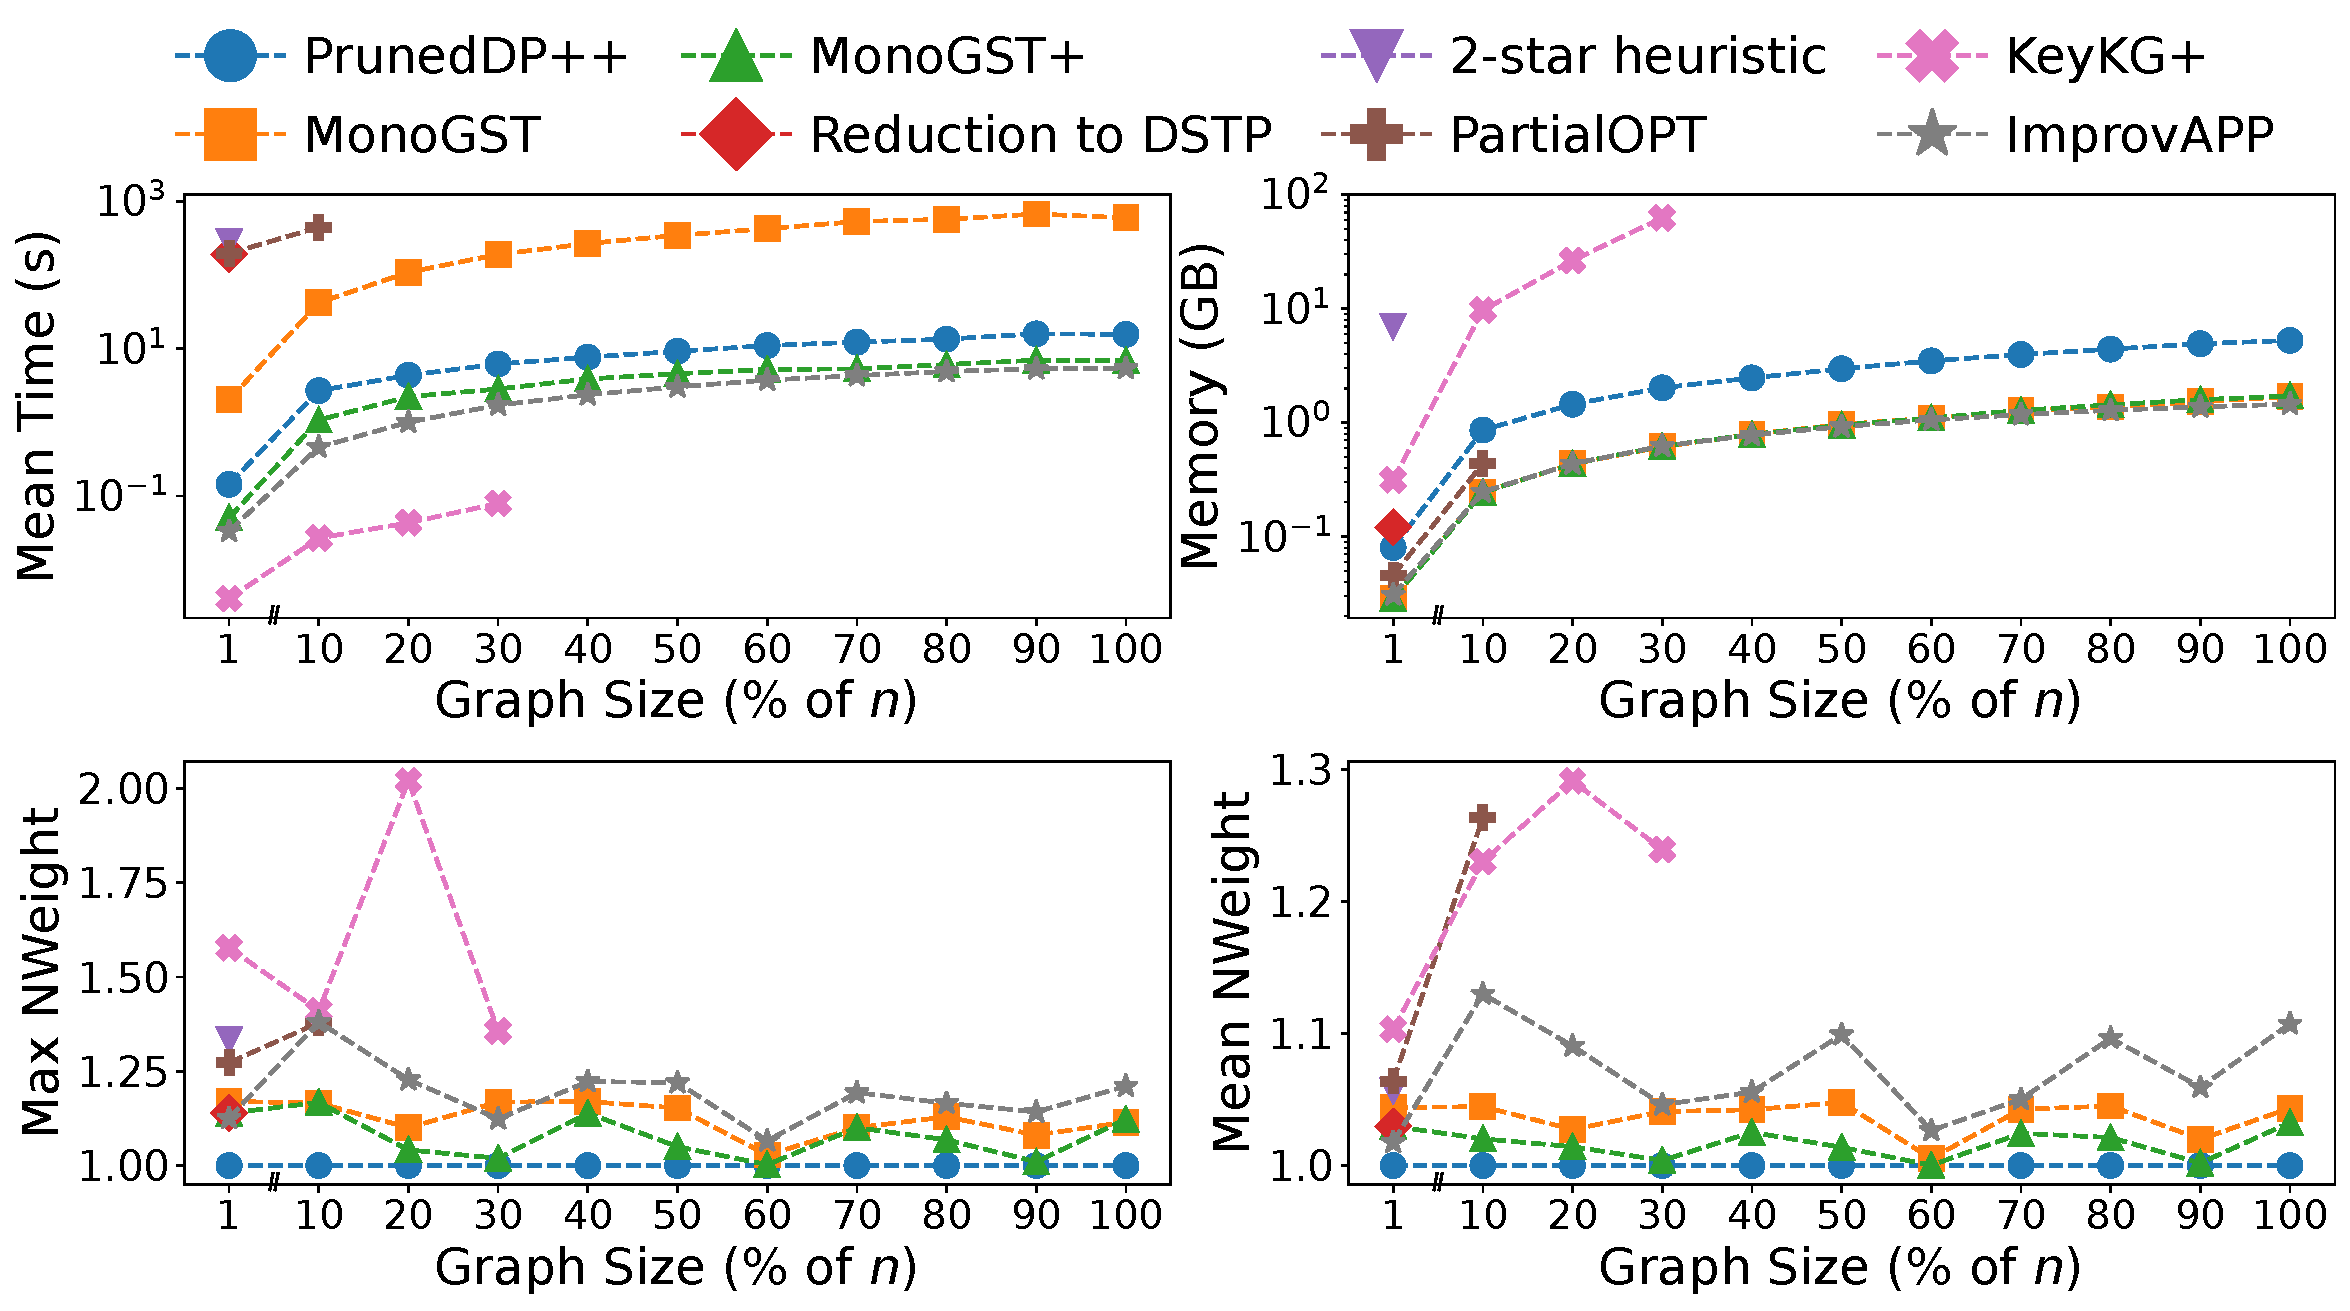
\includegraphics[width=\linewidth]{fig/subgraph/combined_metrics_2x2.pdf}
    \caption{Scalability analysis.}
    \label{fig: subgraph}
\end{figure}

\subsubsection{Experimental Results}

\dew{Figure~\ref{fig: subgraph} shows, for each algorithm on each graph, its mean running time, memory used, and maximum and mean NWeights over all GSTP instances.}

\dew{\textbf{Efficiency Results (Running Time and Memory Use).}
ImprovAPP and our \ImprovPTS are the fastest index-free algorithms and have the lowest memory use. Crucially, their time and space increase slowly with~$n$.
% The running time of \ImprovPTS increases smoothly from 0.05~seconds on the smallest subgraph to 6.82~seconds on the largest.
% The memory usage of \ImprovPTS increases from 0.029~GB to 1.716~GB.
Other algorithms that exhibit comparable scalability though slower include PrunedDP++ and our \Basic.}

\dew{The remaining algorithms show scalability limitations and their curves terminate early. The index building in KeyKG$^+$ uses a vast volume of memory and is complete within 24~hours only for the smallest four graphs. The reduction-to-DSTP approach, the 2‑star heuristic, and PartialOPT encounter timeouts on all GSTP instances on all but the smallest one or two graphs. The 2‑star heuristic also has the highest memory use, more than~7GB for the smallest graph.}

\dew{\textbf{Effectiveness Results (NWeight).}
For all approximation algorithms, their NWeights fluctuate when graph expands. On almost all graphs, our 2-star-based algorithms output better results than ImprovAPP and KeyKG$^+$ based on 1-star.
% ImprovPTS attains the lowest mean NWeight on 10 of the 11 subgraphs, and the lowest maximum NWeight on 7, with one additional tie. Its mean and maximum NWeights are always at most 1.033 and 1.167, respectively.
}

% Respond Reviewer #5 R5: In particular, the authors should clarify how timeout cases are handled in quality comparisons, and report whether the conclusions change under an evaluation that includes all instances (for example, by treating timeout cases conservatively). In addition, if polylogarithmic-approximation methods are too expensive for the full datasets, they should be evaluated on smaller graphs/subgraphs or otherwise discussed more explicitly to better position the proposed method.
\dew{\textbf{Concluding Remarks.}
Our \ImprovPTS is among the highest scalable algorithms and its finer solution quality remains consistent across different graph sizes, strengthening its practicality.}

% Respond Reviewer #4 R3: Although the authors vary the number of groups (g) and the average group size (f), Table 3 presents only aggregate results, failing to show how these parameters affect algorithm performance independently. The authors should include detailed sensitivity analyses, such as plots of runtime and NWeight against varying g and f, to demonstrate the algorithm's robustness across different query configurations.
\subsection{Robustness Analysis}
\label{subsec: sensitivity}

\dew{We analyzed how the number of groups~$g$ and the average group size~$f$ affect the performance of our \ImprovPTS.}

\subsubsection{Parameter Settings}

\dew{On DBLP, we followed the query generation scheme described in Section~\ref{sec:datasets} to generate more queries under extended parameter ranges: varying $g\in\{5,10,\dots,50\}$ with $f=200$, and varying $f\in\{200,400,\dots,2000\}$ with $g=5$.}
% again using 10 random queries per setting.

\begin{figure}[t]
    \centering
    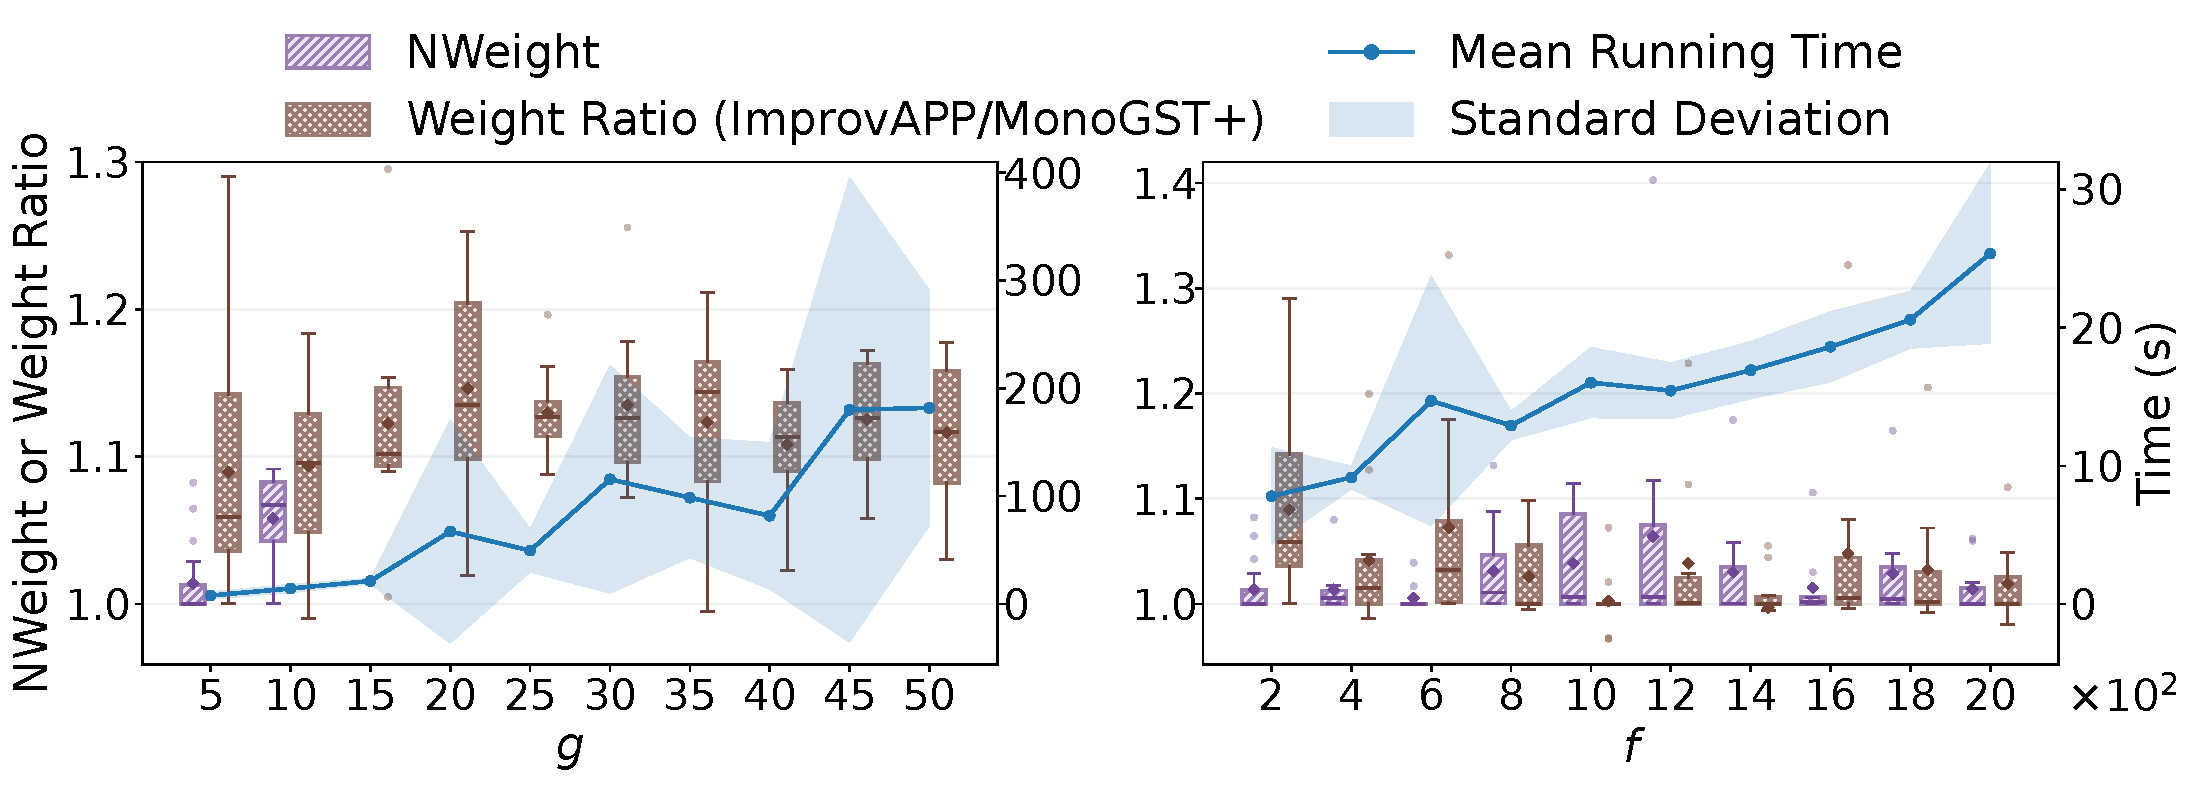
\includegraphics[width=\linewidth]{fig/big_g_f/DBLP_gfv_three_metrics_combined.pdf}
    \caption{Robustness analysis of \ImprovPTS.}
    \label{fig: sens_gf}
\end{figure}

\subsubsection{Experimental Results}

\dew{Figure~\ref{fig: sens_gf} plots the distributions of running time and NWeight of \ImprovPTS over all GSTP instances in each parameter setting. For $g>10$, the exact solver could not find a minimum-weight GST in reasonable time since its time complexity is exponential in~$g$, so NWeight became unavailable; compensating for that, we also calculated the ratio of the weight of the GST computed by our main baseline ImprovAPP to that by \ImprovPTS.}

% Respond Reviewer #2 R1: In the experiments, the values of g are set to [5, 8] which are too small. This setting is not super meaningful to me.
% To see this, according to Table 1, if g is such a small constant, the running time of ImprovAPP is bounded by O(m + n^2) which is better than the one of MonoGST+ O(nm + n^2). Moreover, in this case, the approximation ratios of both these algorithms are considered O(1).
% These assertions are also evidenced by the experimental results. In Table 3, the running time of ImprovAPP is faster than MonoGST+ in most of datasets (except for LinkedMDB) and its average NWeight is competitive to that of MonoGST+, where both of them are very close to 1.
% Therefore, from these experimental results, the effectiveness of MonoGST+ is less significant.

% Respond Reviewer #2 R3(?): As mentioned in O1, the practical performance of MonoGST+ seems not substantially better than the existing SOTA ImprovAPP.
% The authors need to design experiments to show the superiority of their algorithm.

% Respond Reviewer #5 R1: The revision should analyze how performance changes with the number of groups (g), ...
% Respond Reviewer #2 R2. The dedicated experimental study on impact of the average group sizes f is missing. It is unclear that why f is set to {200, 400, 800, 1600}.
% Experiments on f is needed. The impact of a large g with small f is unclear from the current experimental results.
\dew{\textbf{Efficiency Results (Running Time).}
In general, the mean running time increases near proportionally to~$g$ and~$f$, from~7.80 to 181.85~seconds when $g$~increases from~5 to~50, and from~7.80 to 25.37~seconds when $f$~increases from~200 to~2,000.}

\dew{\textbf{Effectiveness Results (NWeight).}
The mean NWeight fluctuates between~1.006 and~1.064 when $f$~changes from~200 to~2,000. It is also small when $g \leq 10$. For larger values of~$g$ such that NWeight is not calculable, the mean weight ratio of ImprovAPP to \ImprovPTS is kept between~1.108 and~1.146; it is also mostly above~1 when $f$~changes, showing that \ImprovPTS robustly delivers high-quality solutions and outperforms ImprovAPP.}
% The paired quality ratio is at least~1 on almost all settings and is within 0.4\% of parity in the only slightly unfavorable case.

\dew{\textbf{Concluding Remarks.}
The high accuracy of \ImprovPTS is insensitive to~$g$ and~$f$. Its running time is empirically linear in these parameters, conforming to our theoretical analysis in Section~\ref{sec:improve-time}.}

\begin{table}[t]
    \centering
    \caption{Ablation study of \ImprovPTS.}
    \label{table: abl}
    \small
    \begin{tabular}{l r @{\hspace{2pt}} l c r @{\hspace{2pt}} l}
    \toprule
    \multirow{2}{*}{Algorithm}
    & \multicolumn{2}{c}{\multirow{2}{*}{Mean Time (s) ${\scriptstyle\downarrow}$}}
    & \multicolumn{3}{c}{NWeight ${\scriptstyle\downarrow}$} \\
    \cline{4-6}
    & & & Max & \multicolumn{2}{c}{Mean}\\
    \midrule
%    \multicolumn{6}{c}{\emph{Experimental results on Toronto}} \\
     \ImprovPTS \emph{on Toronto} & 0.085 & \scriptsize{$\pm$ 0.041} & 1.417 & 1.026 & \scriptsize{$\pm$ 0.051} \\
     w/o suspension & 7.884 & \scriptsize{$\pm$ 5.873} & 1.417 & 1.025 & \scriptsize{$\pm$ 0.050}\\
     w/o suspension \& pruning & 11.819 & \scriptsize{$\pm$ 9.734} & 1.417 & 1.025 & \scriptsize{$\pm$ 0.049} \\
     w/o re-selection & 0.088 & \scriptsize{$\pm$ 0.043} & 1.417 & 1.056 & \scriptsize{$\pm$ 0.069} \\
    \dew{median group} & 0.101 & \scriptsize{$\pm$ 0.041} & 1.417 & 1.026 & \scriptsize{$\pm$ 0.051} \\
    \dew{largest group} & 0.101 & \scriptsize{$\pm$ 0.041} & 1.417 & 1.026 & \scriptsize{$\pm$ 0.051} \\
    % \ImprovPTS \scriptsize{(medium-group)} & 0 & 0.101 & \scriptsize{$\pm$ 0.041} & 1.417 & 1.026 & \scriptsize{$\pm$ 0.051} \\
    % \ImprovPTS \scriptsize{(max-group)} & 0 & 0.101 & \scriptsize{$\pm$ 0.041} & 1.417 & 1.026 & \scriptsize{$\pm$ 0.051} \\
    \hline
%    \multicolumn{6}{c}{\emph{Experimental results on MovieLens}} \\
     \ImprovPTS \emph{on MovieLens} & 1.599 & \scriptsize{$\pm$ 0.316} & 1.192 & 1.015 & \scriptsize{$\pm$ 0.035}\\
     w/o suspension & 49.986 & \scriptsize{$\pm$ 35.506} & 1.192 & 1.015 & \scriptsize{$\pm$ 0.035} \\
     w/o suspension \& pruning & 51.145 & \scriptsize{$\pm$ 36.323} & 1.192 & 1.015 & \scriptsize{$\pm$ 0.035} \\
     w/o re-selection & 1.649 & \scriptsize{$\pm$ 0.274} & 1.192 & 1.025 & \scriptsize{$\pm$ 0.042} \\
    \dew{median group} & 1.653 & \scriptsize{$\pm$ 0.303} & 1.192 & 1.015 & \scriptsize{$\pm$ 0.035} \\
    \dew{largest group} & 1.600 & \scriptsize{$\pm$ 0.269} & 1.192 & 1.015 & \scriptsize{$\pm$ 0.035} \\
    \hline
%    \multicolumn{6}{c}{\emph{Experimental results on DBLP}} \\
     \ImprovPTS \emph{on DBLP} & 15.876 & \scriptsize{$\pm$ 8.242} & 1.209 & 1.032 & \scriptsize{$\pm$ 0.042}\\
     w/o suspension & 1700.880 & \scriptsize{$\pm$ 1247.202} & 1.209 & 1.031 & \scriptsize{$\pm$ 0.041}\\
     w/o suspension \& pruning & 2394.501 & \scriptsize{$\pm$ 1834.009} & 1.209 & 1.031 & \scriptsize{$\pm$ 0.041} \\
     w/o re-selection & 16.669 & \scriptsize{$\pm$ 10.110} & 1.241 & 1.058 & \scriptsize{$\pm$ 0.053}\\
    \dew{median group} & 16.261 & \scriptsize{$\pm$ 8.354} & 1.209 & 1.032 & \scriptsize{$\pm$ 0.042} \\
    \dew{largest group} & 16.275 & \scriptsize{$\pm$ 8.524} & 1.209 & 1.032 & \scriptsize{$\pm$ 0.042} \\
    \midrule
%    \multicolumn{6}{c}{\emph{Experimental results on LinkedMDB}} \\
     \ImprovPTS \emph{on LinkedMDB} & 0.756 & \scriptsize{$\pm$ 0.671} & 1.223 & 1.040 & \scriptsize{$\pm$ 0.057} \\
     w/o suspension & 1.544 & \scriptsize{$\pm$ 1.684} & 1.223 & 1.038 & \scriptsize{$\pm$ 0.055}\\
     w/o suspension \& pruning & 1.572 & \scriptsize{$\pm$ 1.732} & 1.223 & 1.038 & \scriptsize{$\pm$ 0.055}\\
     w/o re-selection & 0.753 & \scriptsize{$\pm$ 0.667} & 1.261 & 1.053 & \scriptsize{$\pm$ 0.068}\\
    \dew{median group} & 0.763 & \scriptsize{$\pm$ 0.678} & 1.246 & 1.034 & \scriptsize{$\pm$ 0.055} \\
    \dew{largest group} & 0.761 & \scriptsize{$\pm$ 0.677} & 1.246 & 1.034 & \scriptsize{$\pm$ 0.055} \\
    \hline
%    \multicolumn{6}{c}{\emph{Experimental results on DBpedia}} \\
     \ImprovPTS \emph{on DBpedia} & 7.717 & \scriptsize{$\pm$ 3.538} & 1.204 & 1.012 & \scriptsize{$\pm$ 0.029}\\
     w/o suspension & 39.992 & \scriptsize{$\pm$ 107.420} & 1.204 & 1.012 & \scriptsize{$\pm$ 0.029}\\
     w/o suspension \& pruning & 41.697 & \scriptsize{$\pm$ 110.882} & 1.204 & 1.012 & \scriptsize{$\pm$ 0.028}\\
     w/o re-selection & 7.560 & \scriptsize{$\pm$ 3.447} & 1.204 & 1.016 & \scriptsize{$\pm$ 0.032}\\
    \dew{median group} & 7.853 & \scriptsize{$\pm$ 3.566} & 1.204 & 1.012 & \scriptsize{$\pm$ 0.029} \\
    \dew{largest group} & 7.797 & \scriptsize{$\pm$ 3.560} & 1.204 & 1.012 & \scriptsize{$\pm$ 0.029} \\
    \bottomrule
    \end{tabular}
\end{table}

\subsection{Ablation Study}
\label{subsec: able}

\subsubsection{Variant Settings}

We conducted an ablation study by implementing and comparing five variants of \ImprovPTS, aiming to isolate and quantify the effects of its key components.

The variant \textbf{w/o suspension} replaces our suspendable Dijkstra's algorithm (Section~\ref{subsec: sec_dub}) with the standard Dijkstra's algorithm to compute SSSP from each root $r \in K_1$ in a manner identical to that in \Basic (line~10).
The variant \textbf{w/o suspension \& pruning} further disables our prefix pruning (Section~\ref{subsec: mono_upt}) and enumerates each prefix~$p$ from~2 to~$g$ in a manner identical to that in \Basic (line~14).
The variant \textbf{w/o re-selection} replaces our path re-selection (Section~\ref{subsec: sec_rebuild}) with the naive method for converting a 2-star into a GST described in Section~\ref{subsec: 2-star} in a manner identical to that in \Basic (lines~19--21).
Note that suspension and prefix pruning mainly optimize running time, while path re-selection focuses on solution quality, addressing different aspects of performance.

\dew{\Improved enumerates the vertices in the smallest group as the root of a 2-star (line~1). Differently, the variants \textbf{median group} and \textbf{largest group} choose a group of median size and the largest group as~$K_1$ to enumerate, respectively.}

\subsubsection{Experimental Results}
\label{subsubsec: abl_result}
Table~\ref{table: abl} shows, for each variant on each dataset, its mean running time, and maximum and mean NWeights over all GSTP instances. For precisely reflecting performance difference, we removed per-run time limit from this ablation study.

% Respond Reviewer #5 R1: The revision should..., quantify the benefit of early termination in suspendable Dijkstra (e.g., visited nodes/work saved versus full SSSP), and evaluate the effect of prefix pruning. (最后半句在 Detailed Evaluation 里面说 The effectiveness of prefix pruning is not evaluated as a function of g. 还没加）
\textbf{Efficiency Results (Running Time).}
The suspendability mechanism is the key driver behind the efficiency of \ImprovPTS. It enables speedups of 1--2 orders of magnitude on Toronto, MovieLens, and DBLP, and $2\times$--$5\times$ on LinkedMDB and DBpedia. \dew{With suspendability on different datasets, only an average of 0.02\%--20\% of all vertices are visited when Dijkstra's algorithm is terminated.}

Prefix pruning provides both theoretical and empirical benefits: it reduces the time complexity by a factor of~$g$, and produces consistent speedups across all datasets, up to 29\%--33\% on Toronto and DBLP.
% 总体而言，g 越大增量越多（括号里面举个例子，当 g 从多少到多少 在某个数据集上）
\dew{The benefit becomes more pronounced as $g$~increases, e.g.,~from~21\% to~42\% as $g$~increases from~5 to~8 on Toronto.}

\dew{Switching from the smallest group to the median or largest group leads to consistent increases in running time, up to~19\% on Toronto.}

\textbf{Effectiveness Results (NWeight).}
Path re-selection yields consistent, though modest, quality improvements on all datasets, up to 2\%--3\% reduction in mean NWeight on Toronto and DBLP. Incurring negligible time cost, it represents a net-positive trade-off between effectiveness and efficiency.

\dew{Enumerating the smallest, median, or largest group has little effect on solution quality on most datasets.}

% 使用 suspensio 后实际访问的节点的平均比例
% DBLP:      0.0009301625
% DBpedia:   0.0585949977
% LinkedMDB: 0.1961901100
% MovieLens: 0.0002347000
% Toronto:   0.0007252625

% (w/o suspension & pruning - w/o suspension) / w/o suspension & pruning 不同 g 的 结果
% DBLP
%   g=5: 0.1873611037
%   g=6: 0.2412399713
%   g=7: 0.3068331645
%   g=8: 0.3628756823
% DBpedia
%   g=1: -0.3333333333  skipped_zero=1
%   g=2: -0.0090308388
%   g=3: -0.0001541120
%   g=4: 0.0155753004
%   g=5: 0.0201601114
%   g=6: 0.0313407780
%   g=7: 0.0701080392
%   g=8: 0.0895480933
%   g=9: 0.1030067716
%   g=10: 0.1083023208
% LinkedMDB
%   g=1: -0.0968253968  skipped_zero=5
%   g=2: -0.0376935060
%   g=3: -0.0279413468
%   g=4: 0.0386849984
%   g=5: -0.0015366147
%   g=6: -0.0675875087
%   g=7: -0.0019840130
%   g=8: 0.0341245371
%   g=9: 0.0717124332
%   g=10: 0.0146946877
% MovieLens
%   g=5: 0.0208141968
%   g=6: 0.0188620342
%   g=7: 0.0268043835
%   g=8: 0.0319513820
% Toronto
%   g=5: 0.2139474811
%   g=6: 0.3015960823
%   g=7: 0.3539243170
%   g=8: 0.4153350093

\textbf{Concluding Remarks.}
In summary, all three optimizations integrated into \ImprovPTS collectively establish its superiority over \Basic in terms of efficiency and effectiveness. These novel techniques enable \ImprovPTS to achieve state-of-the-art performance among approximate GST algorithms. \dew{It is also cost-effective to enumerate the vertices in the smallest group as the root of a 2-star.}